% Компилировать XeLaTeX (в Overleaf: Menu → Compiler → XeLaTeX).
% В проект Overleaf загрузить всю папку docs/report: report.tex, images/, code/.
\documentclass[a4paper,12pt]{article}

\usepackage{fontspec}
\usepackage[russian]{babel}
% Шрифты Computer Modern Unicode (есть в TeX Live и MiKTeX), подключены по имени файла
\setmainfont{cmunrm.otf}[BoldFont=cmunbx.otf, ItalicFont=cmunti.otf, BoldItalicFont=cmunbi.otf]
\setsansfont{cmunss.otf}[BoldFont=cmunsx.otf, ItalicFont=cmunsi.otf, BoldItalicFont=cmunso.otf]
\setmonofont{cmuntt.otf}[BoldFont=cmuntb.otf, ItalicFont=cmunit.otf, BoldItalicFont=cmuntx.otf]

\usepackage[left=25mm,right=15mm,top=20mm,bottom=20mm]{geometry}
\usepackage{graphicx}
\usepackage{pdflscape}
\usepackage{float}
\usepackage{caption}
\usepackage{xcolor}
\usepackage{listings}
\usepackage{enumitem}
\usepackage{booktabs}
\usepackage{tabularx}
\usepackage{indentfirst}
\usepackage[hidelinks]{hyperref}

\setlength{\parindent}{1.25cm}
\linespread{1.15}
\setlist{nosep}

% Ссылка на репозиторий — заменить на свою
\newcommand{\repourl}{https://github.com/USERNAME/study-groups}

\definecolor{codebg}{RGB}{248,248,248}
\definecolor{codekw}{RGB}{0,0,160}
\definecolor{codecomment}{RGB}{0,120,0}
\definecolor{codestring}{RGB}{160,40,40}

\lstset{
  basicstyle=\ttfamily\footnotesize,
  keywordstyle=\color{codekw}\bfseries,
  commentstyle=\color{codecomment}\itshape,
  stringstyle=\color{codestring},
  backgroundcolor=\color{codebg},
  frame=single,
  rulecolor=\color{gray!50},
  breaklines=true,
  breakatwhitespace=false,
  columns=fullflexible,
  keepspaces=true,
  showstringspaces=false,
  numbers=left,
  numberstyle=\tiny\color{gray},
  tabsize=4,
  captionpos=t,
  extendedchars=true
}

\lstdefinelanguage{TypeScript}{
  language=Java,
  morekeywords={const,let,function,export,import,from,type,interface,async,await,as,of},
  morestring=[b]',
  morestring=[b]`
}

\lstdefinelanguage{PGSQL}{
  language=SQL,
  morekeywords={RETURNS,SETOF,LANGUAGE,STABLE,DECLARE,BEGIN,END,RETURN,QUERY,RAISE,EXCEPTION,
    IF,THEN,FOUND,USING,ERRCODE,RETURNING,INTO,GENERATED,ALWAYS,IDENTITY,BIGINT,REAL,DOUBLE,
    PRECISION,TEXT,VARCHAR,INTEGER,TIMESTAMPTZ,CONSTRAINT,CHECK,REFERENCES,REPLACE,FUNCTION,
    TABLE,INDEX,DEFAULT,ROWTYPE,plpgsql},
  sensitive=false
}

\renewcommand{\lstlistingname}{Листинг}
\captionsetup{font=small}

\begin{document}

\begin{titlepage}
\centering
{\small
Федеральное государственное автономное образовательное учреждение высшего образования\\
«Санкт-Петербургский национальный исследовательский университет\\
информационных технологий, механики и оптики»\\[0.5cm]
Факультет Программной Инженерии и Компьютерной техники\\[2cm]
}

{\Large\bfseries Лабораторная работа №1 по дисциплине «Информационные системы»\\[0.5cm]}
{\large Информационная система для управления объектами класса StudyGroup\\[2cm]}

\vspace{4 cm}
\begin{flushright}
\begin{tabular}{l}
Выполнил студент 3-го курса\\
Сушко Александр\\
Группа Р3317\\
Табельный номер 467647\\[1cm]
Проверил\\
Николаев Владимир Вячеславович\\
\end{tabular}
\end{flushright}

\vfill
Санкт-Петербург\\2026 год
\end{titlepage}

\tableofcontents
\newpage

% =====================================================================
\section{Текст задания}

Реализовать информационную систему, которая позволяет взаимодействовать с объектами класса \texttt{StudyGroup}, описание которого приведено ниже:

\begin{lstlisting}[language=Java, caption={Описание классов предметной области}, numbers=none]
public class StudyGroup {
    private Long id; //Поле не может быть null, Значение поля должно быть больше 0, Значение этого поля должно быть уникальным, Значение этого поля должно генерироваться автоматически
    private String name; //Поле не может быть null, Строка не может быть пустой
    private Coordinates coordinates; //Поле не может быть null
    private java.time.ZonedDateTime creationDate; //Поле не может быть null, Значение этого поля должно генерироваться автоматически
    private int studentsCount; //Значение поля должно быть больше 0
    private int expelledStudents; //Значение поля должно быть больше 0
    private Long transferredStudents; //Значение поля должно быть больше 0, Поле не может быть null
    private FormOfEducation formOfEducation; //Поле не может быть null
    private Long shouldBeExpelled; //Значение поля должно быть больше 0, Поле не может быть null
    private Long averageMark; //Значение поля должно быть больше 0, Поле не может быть null
    private Semester semesterEnum; //Поле не может быть null
    private Person groupAdmin; //Поле может быть null
}
public class Coordinates {
    private Float x; //Поле не может быть null
    private double y;
}
public class Person {
    private String name; //Поле не может быть null, Строка не может быть пустой
    private Color eyeColor; //Поле может быть null
    private Color hairColor; //Поле не может быть null
    private Location location; //Поле может быть null
    private float weight; //Значение поля должно быть больше 0
    private String passportID; //Поле может быть null
    private Country nationality; //Поле может быть null
}
public class Location {
    private float x;
    private double y;
    private String name; //Поле не может быть null
}
public enum FormOfEducation {
    DISTANCE_EDUCATION,
    FULL_TIME_EDUCATION,
    EVENING_CLASSES;
}
public enum Semester {
    THIRD,
    FOURTH,
    SIXTH,
    SEVENTH,
    EIGHTH;
}
public enum Color {
    GREEN,
    WHITE,
    BROWN;
}
public enum Country {
    USA,
    FRANCE,
    SPAIN,
    VATICAN,
    THAILAND;
}
\end{lstlisting}

Разработанная система должна удовлетворять следующим требованиям:
\begin{itemize}
  \item Основное назначение информационной системы "--- управление объектами, созданными на основе заданного в варианте класса.
  \item Необходимо, чтобы с помощью системы можно было выполнить следующие операции с объектами: создание нового объекта, получение информации об объекте по ИД, обновление объекта (модификация его атрибутов), удаление объекта. Операции должны осуществляться в отдельных окнах (интерфейсах) приложения. При получении информации об объекте класса должна также выводиться информация о связанных с ним объектах.
  \item При создании объекта класса необходимо дать пользователю возможность связать новый объект с объектами вспомогательных классов, которые могут быть связаны с созданным объектом и уже есть в системе.
  \item Выполнение операций по управлению объектами должно осуществляться на серверной части (не на клиенте), изменения должны синхронизироваться с базой данных.
  \item На главном экране системы должен выводиться список текущих объектов в виде таблицы (каждый атрибут объекта "--- отдельная колонка в таблице). При отображении таблицы должна использоваться пагинация (если все объекты не помещаются на одном экране).
  \item Нужно обеспечить возможность фильтровать/сортировать строки таблицы, которые показывают объекты (по значениям любой из строковых колонок). Фильтрация элементов должна производиться по неполному совпадению.
  \item Переход к обновлению (модификации) объекта должен быть возможен из таблицы с общим списком объектов и из области с визуализацией объекта (при ее реализации).
  \item При добавлении/удалении/изменении объекта, он должен автоматически появиться/исчезнуть/измениться в интерфейсах у других пользователей, авторизованных в системе.
  \item Если при удалении объекта с ним связан другой объект, связанные объекты должны быть связаны с другим объектом (по выбору пользователя), а изначальный объект удален.
  \item Пользователи должны иметь возможность просмотра всех объектов. Для модификации объекта должно открываться отдельное диалоговое окно. При вводе некорректных значений в поля объекта должны появляться информативные сообщения о соответствующих ошибках.
\end{itemize}

В системе должен быть реализован отдельный пользовательский интерфейс для выполнения специальных операций над объектами:
\begin{itemize}
  \item Вернуть один (любой) объект, значение поля \texttt{expelledStudents} которого является минимальным.
  \item Сгруппировать объекты по значению поля \texttt{id}, вернуть количество элементов в каждой группе.
  \item Вернуть массив объектов, значение поля \texttt{groupAdmin} которых больше заданного.
  \item Отчислить всех студентов указанной группы.
  \item Добавить студента в указанную группу.
\end{itemize}

Представленные операции должны быть реализованы в качестве функций БД, которые необходимо вызывать из уровня бизнес-логики приложения.

Особенности хранения объектов, которые должны быть реализованы в системе:
\begin{itemize}
  \item Организовать хранение данных об объектах в реляционной СУБД (PostgreSQL). Каждый объект, с которым работает ИС, должен быть сохранен в базе данных.
  \item Все требования к полям класса (указанные в виде комментариев к описанию классов) должны быть выполнены на уровне ORM и БД.
  \item Для генерации поля \texttt{id} использовать средства базы данных.
  \item Для подключения к БД на кафедральном сервере использовать хост \texttt{pg}, имя базы данных "--- \texttt{studs}, имя пользователя/пароль совпадают с таковыми для подключения к серверу.
\end{itemize}

При создании системы нужно учитывать следующие особенности организации взаимодействия с пользователем:
\begin{itemize}
  \item Система должна реагировать на некорректный пользовательский ввод, ограничивая ввод недопустимых значений и информируя пользователей о причине ошибки.
  \item Переходы между различными логически обособленными частями системы должны осуществляться с помощью меню.
  \item При добавлении/удалении/изменении объекта, он должен автоматически появиться/исчезнуть/измениться на области у всех других клиентов.
\end{itemize}

При разработке ИС должны учитываться следующие требования:
\begin{itemize}
  \item В качестве основы для реализации ИС необходимо использовать Spring MVC.
  \item Для создания уровня хранения необходимо использовать JPA + EclipseLink.
  \item Разные уровни приложения должны быть отделены друг от друга, разные логические части ИС должны находиться в отдельных компонентах.
\end{itemize}

\newpage
% =====================================================================
\section{UML-диаграммы классов и пакетов}

\subsection{Архитектура приложения}

Система построена по клиент-серверной схеме. Клиентская часть "--- одностраничное приложение на React (TypeScript, Vite), серверная часть "--- приложение на Spring Boot 3 (Spring MVC) с уровнем хранения на JPA + EclipseLink и СУБД PostgreSQL. Клиент обращается к серверу по REST (JSON), а уведомления об изменениях получает по WebSocket (протокол STOMP).

Серверная часть разделена на слои:
\begin{itemize}
  \item \textbf{web} "--- REST-контроллеры и единый обработчик ошибок (\texttt{@RestControllerAdvice});
  \item \textbf{service} "--- бизнес-логика; каждая операция выполняется в транзакции (\texttt{@Transactional});
  \item \textbf{repository} "--- доступ к данным: репозитории Spring Data JPA, динамические запросы на Criteria API, вызов функций БД;
  \item \textbf{domain} "--- JPA-сущности и перечисления;
  \item \textbf{dto}, \textbf{mapper} "--- объекты передачи данных и их преобразование из сущностей;
  \item \textbf{realtime} "--- рассылка событий клиентам после фиксации транзакции;
  \item \textbf{config} "--- настройка EclipseLink, WebSocket и раздачи клиентского приложения;
  \item \textbf{exception} "--- исключения бизнес-уровня.
\end{itemize}

Схема БД, ограничения на поля (\texttt{NOT NULL}, \texttt{CHECK}, внешние ключи) и функции специальных операций создаются миграциями Flyway: версионными \texttt{V1}, \texttt{V3} и повторяемой \texttt{R\_\_special\_operations.sql}, которая перевыполняется при каждом её изменении. Те же ограничения продублированы на уровне ORM аннотациями Bean Validation и \texttt{@Column(nullable = false)}. Поле \texttt{id} генерируется СУБД (\texttt{GENERATED ALWAYS AS IDENTITY}).

Синхронизация клиентов: сервис после изменения данных публикует событие \texttt{EntityChangedEvent}; компонент \texttt{ChangeBroadcaster} с аннотацией \texttt{@TransactionalEventListener(phase = AFTER\_COMMIT)} после успешной фиксации транзакции отправляет событие в топик \texttt{/topic/changes}; клиенты, подписанные на топик, перезапрашивают отображаемые данные.

Исходная диаграмма в формате draw.io: \texttt{uml.drawio}.

\begin{landscape}
\begin{figure}[p]
  \centering
  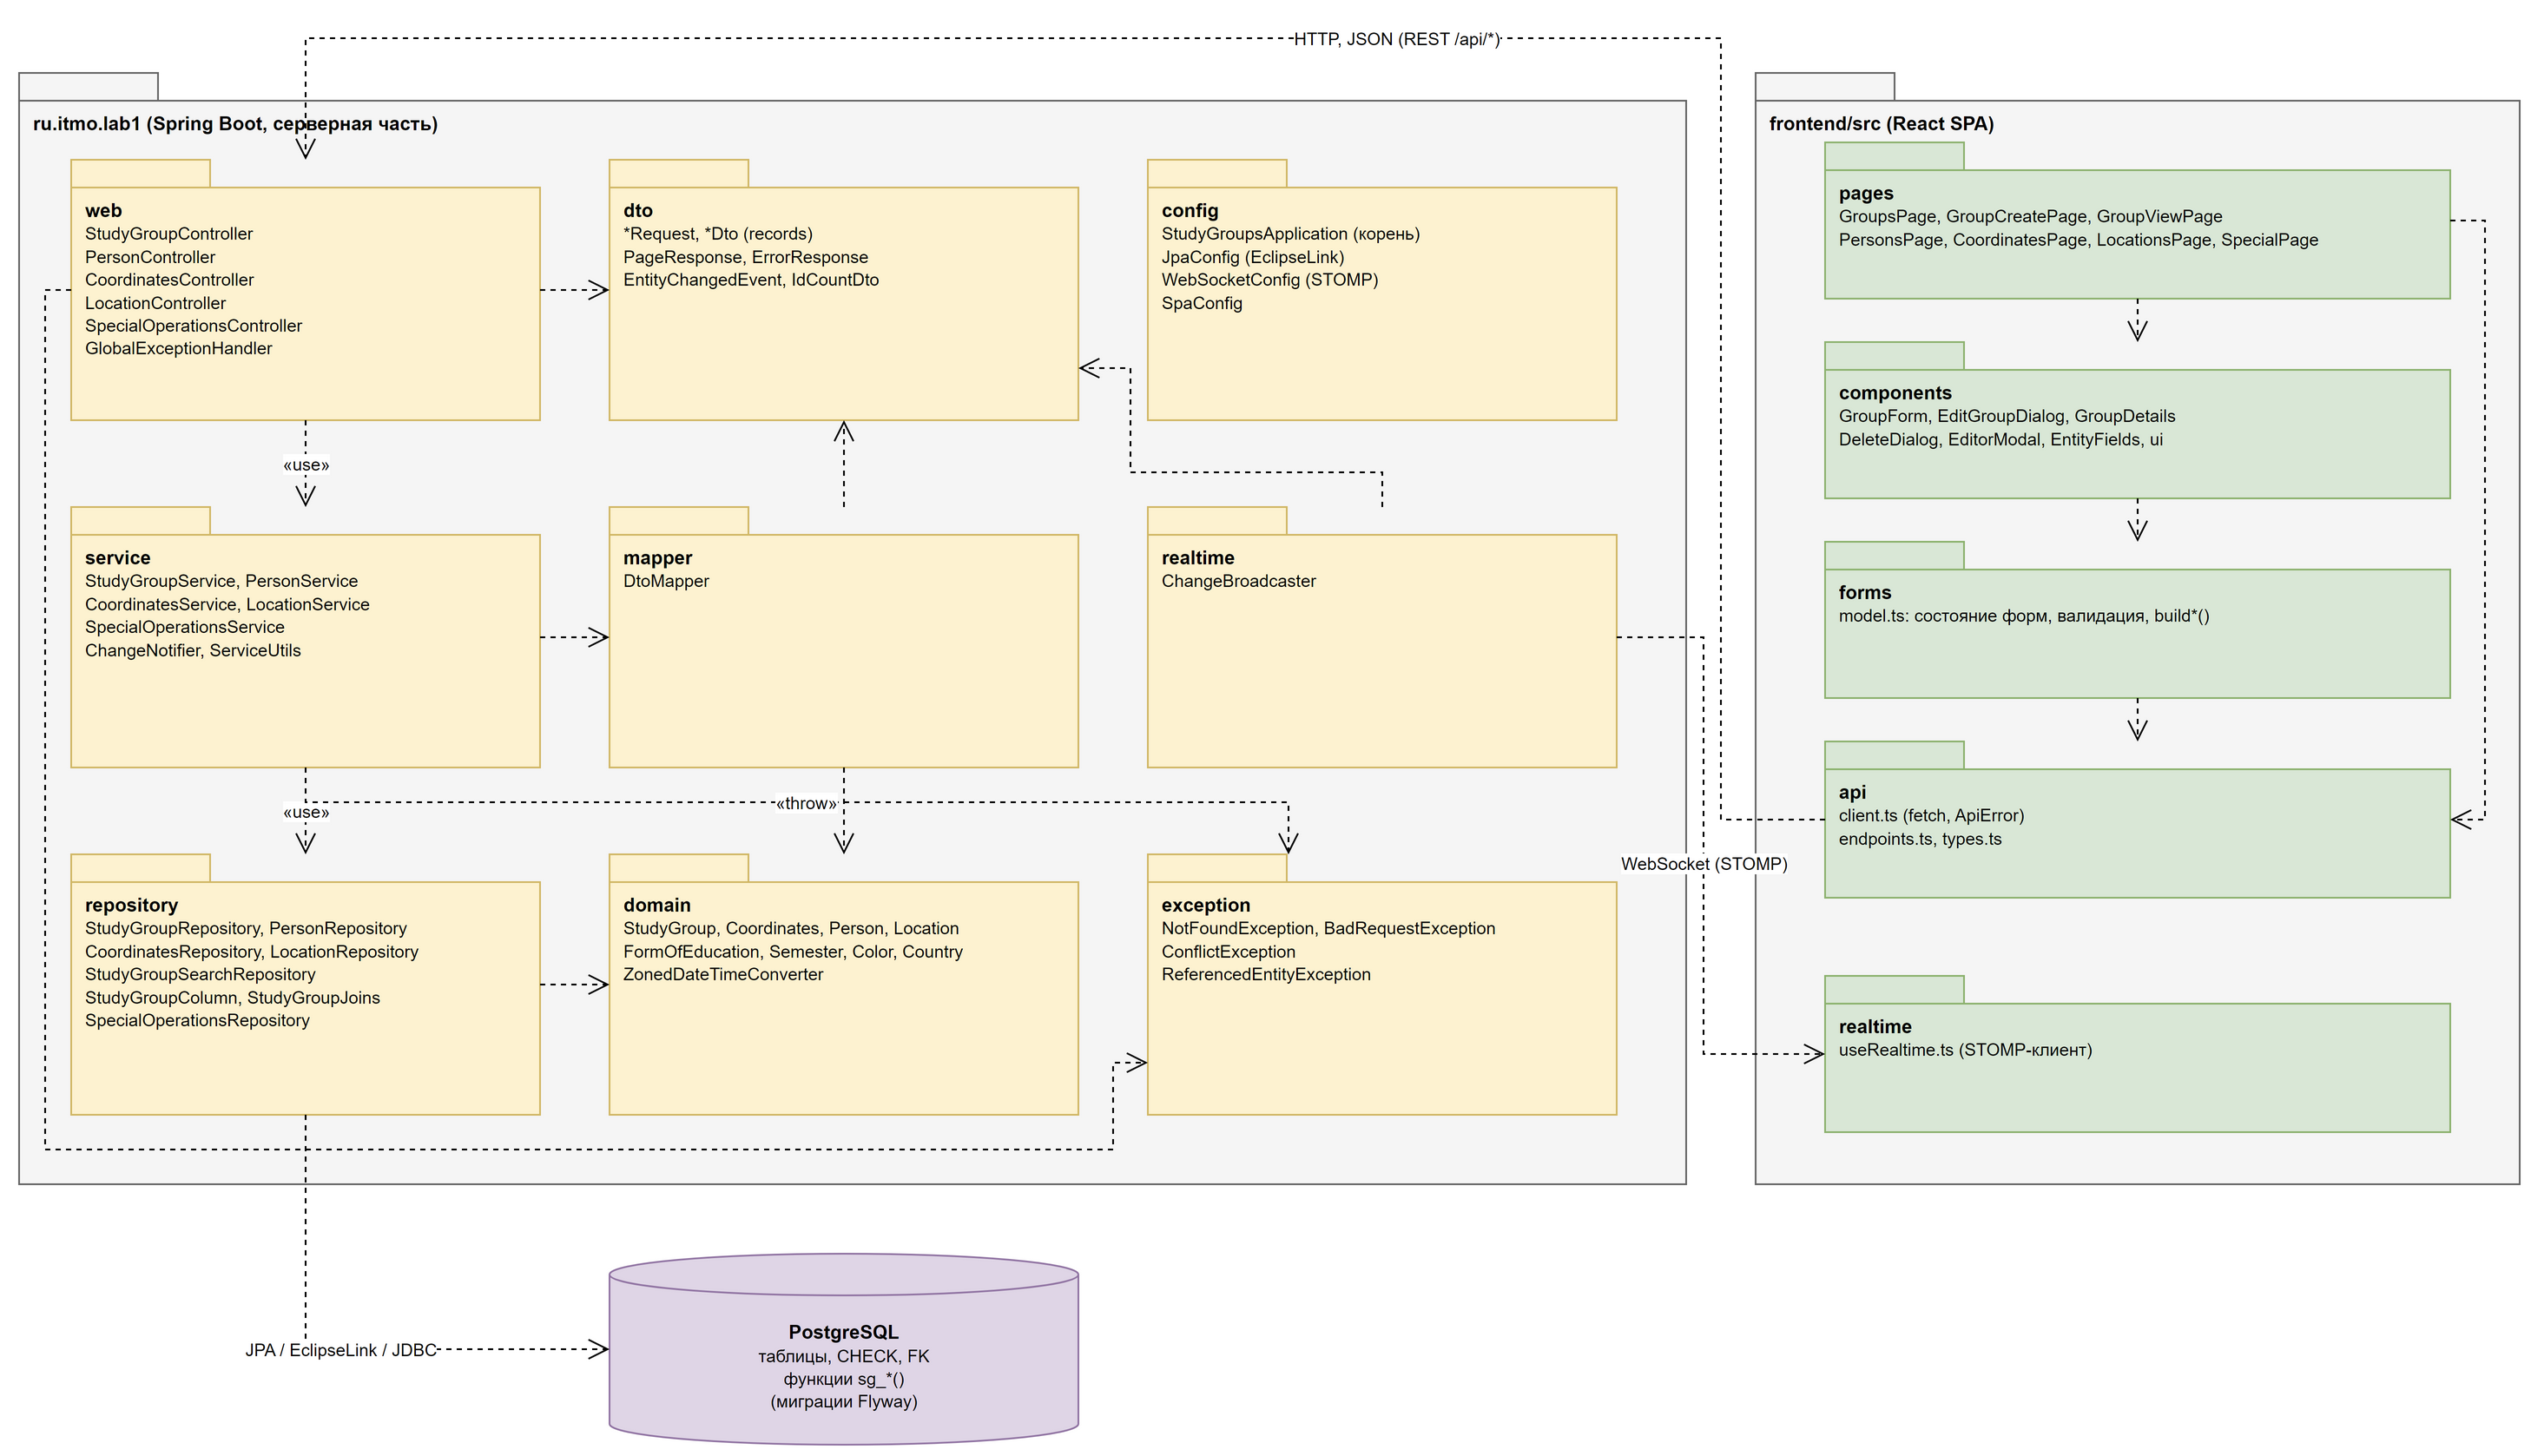
\includegraphics[width=\linewidth,height=0.8\textheight,keepaspectratio]{images/uml-1.png}
  \caption{Диаграмма пакетов}
  \label{fig:packages}
\end{figure}

\begin{figure}[p]
  \centering
  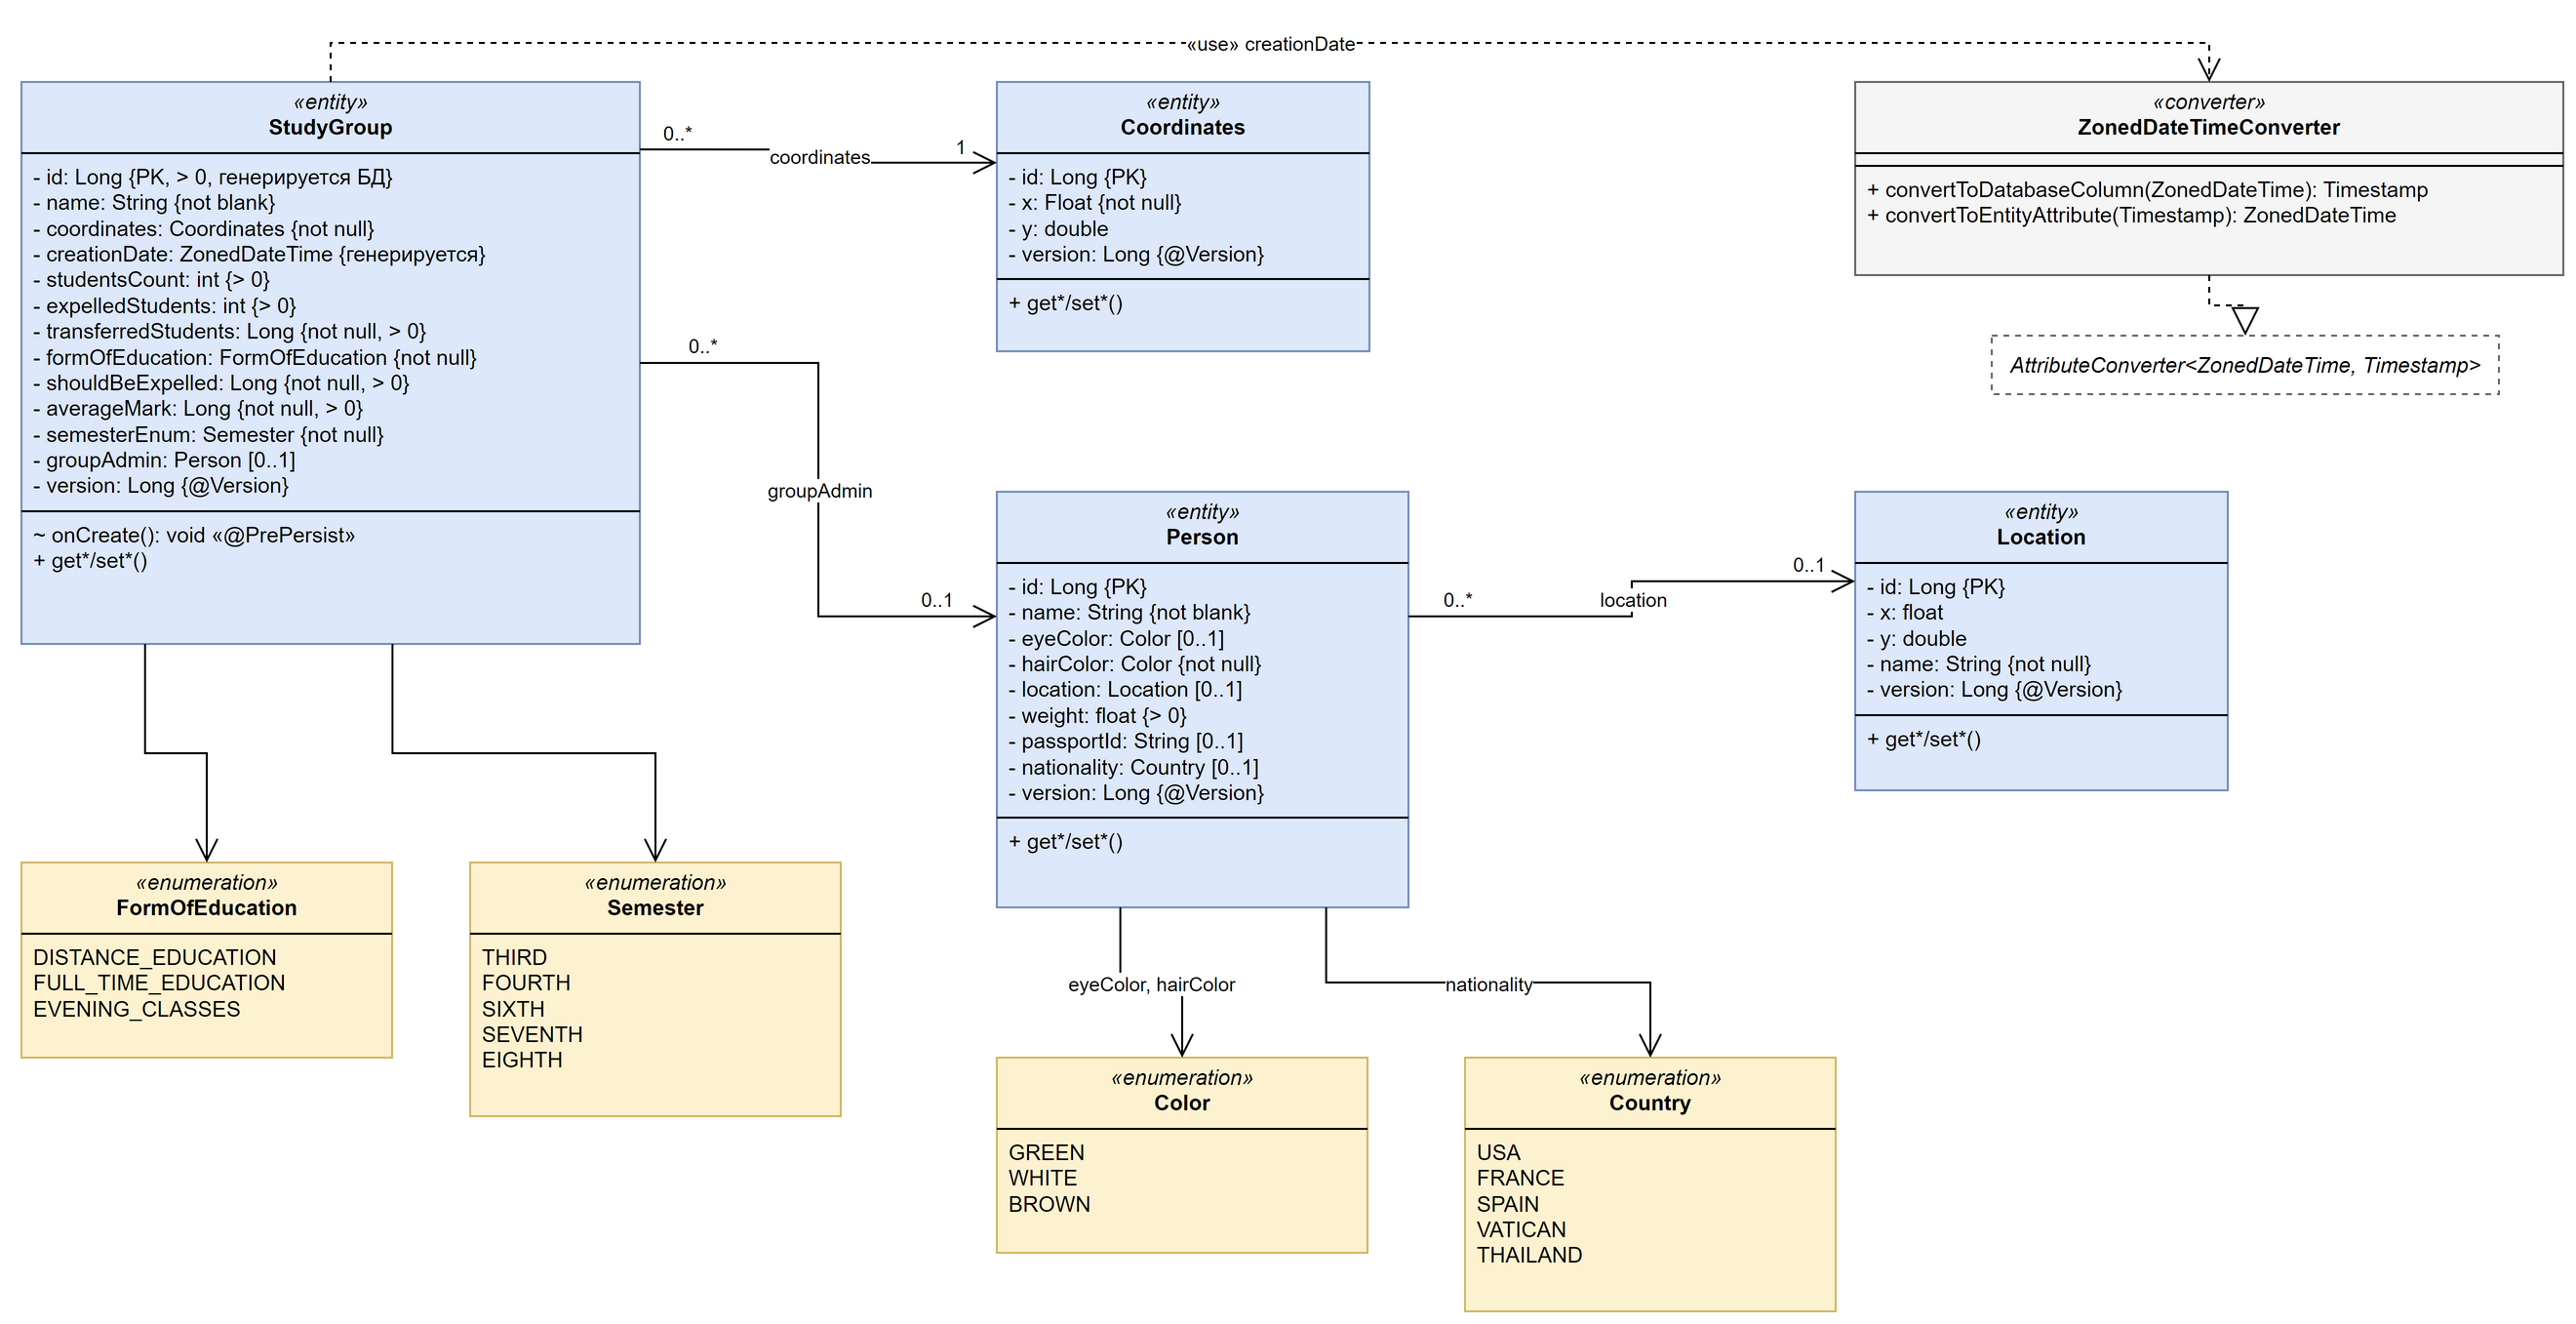
\includegraphics[width=\linewidth,height=0.8\textheight,keepaspectratio]{images/uml-2.png}
  \caption{Диаграмма классов: доменная модель (пакет \texttt{domain})}
  \label{fig:domain}
\end{figure}

\begin{figure}[p]
  \centering
  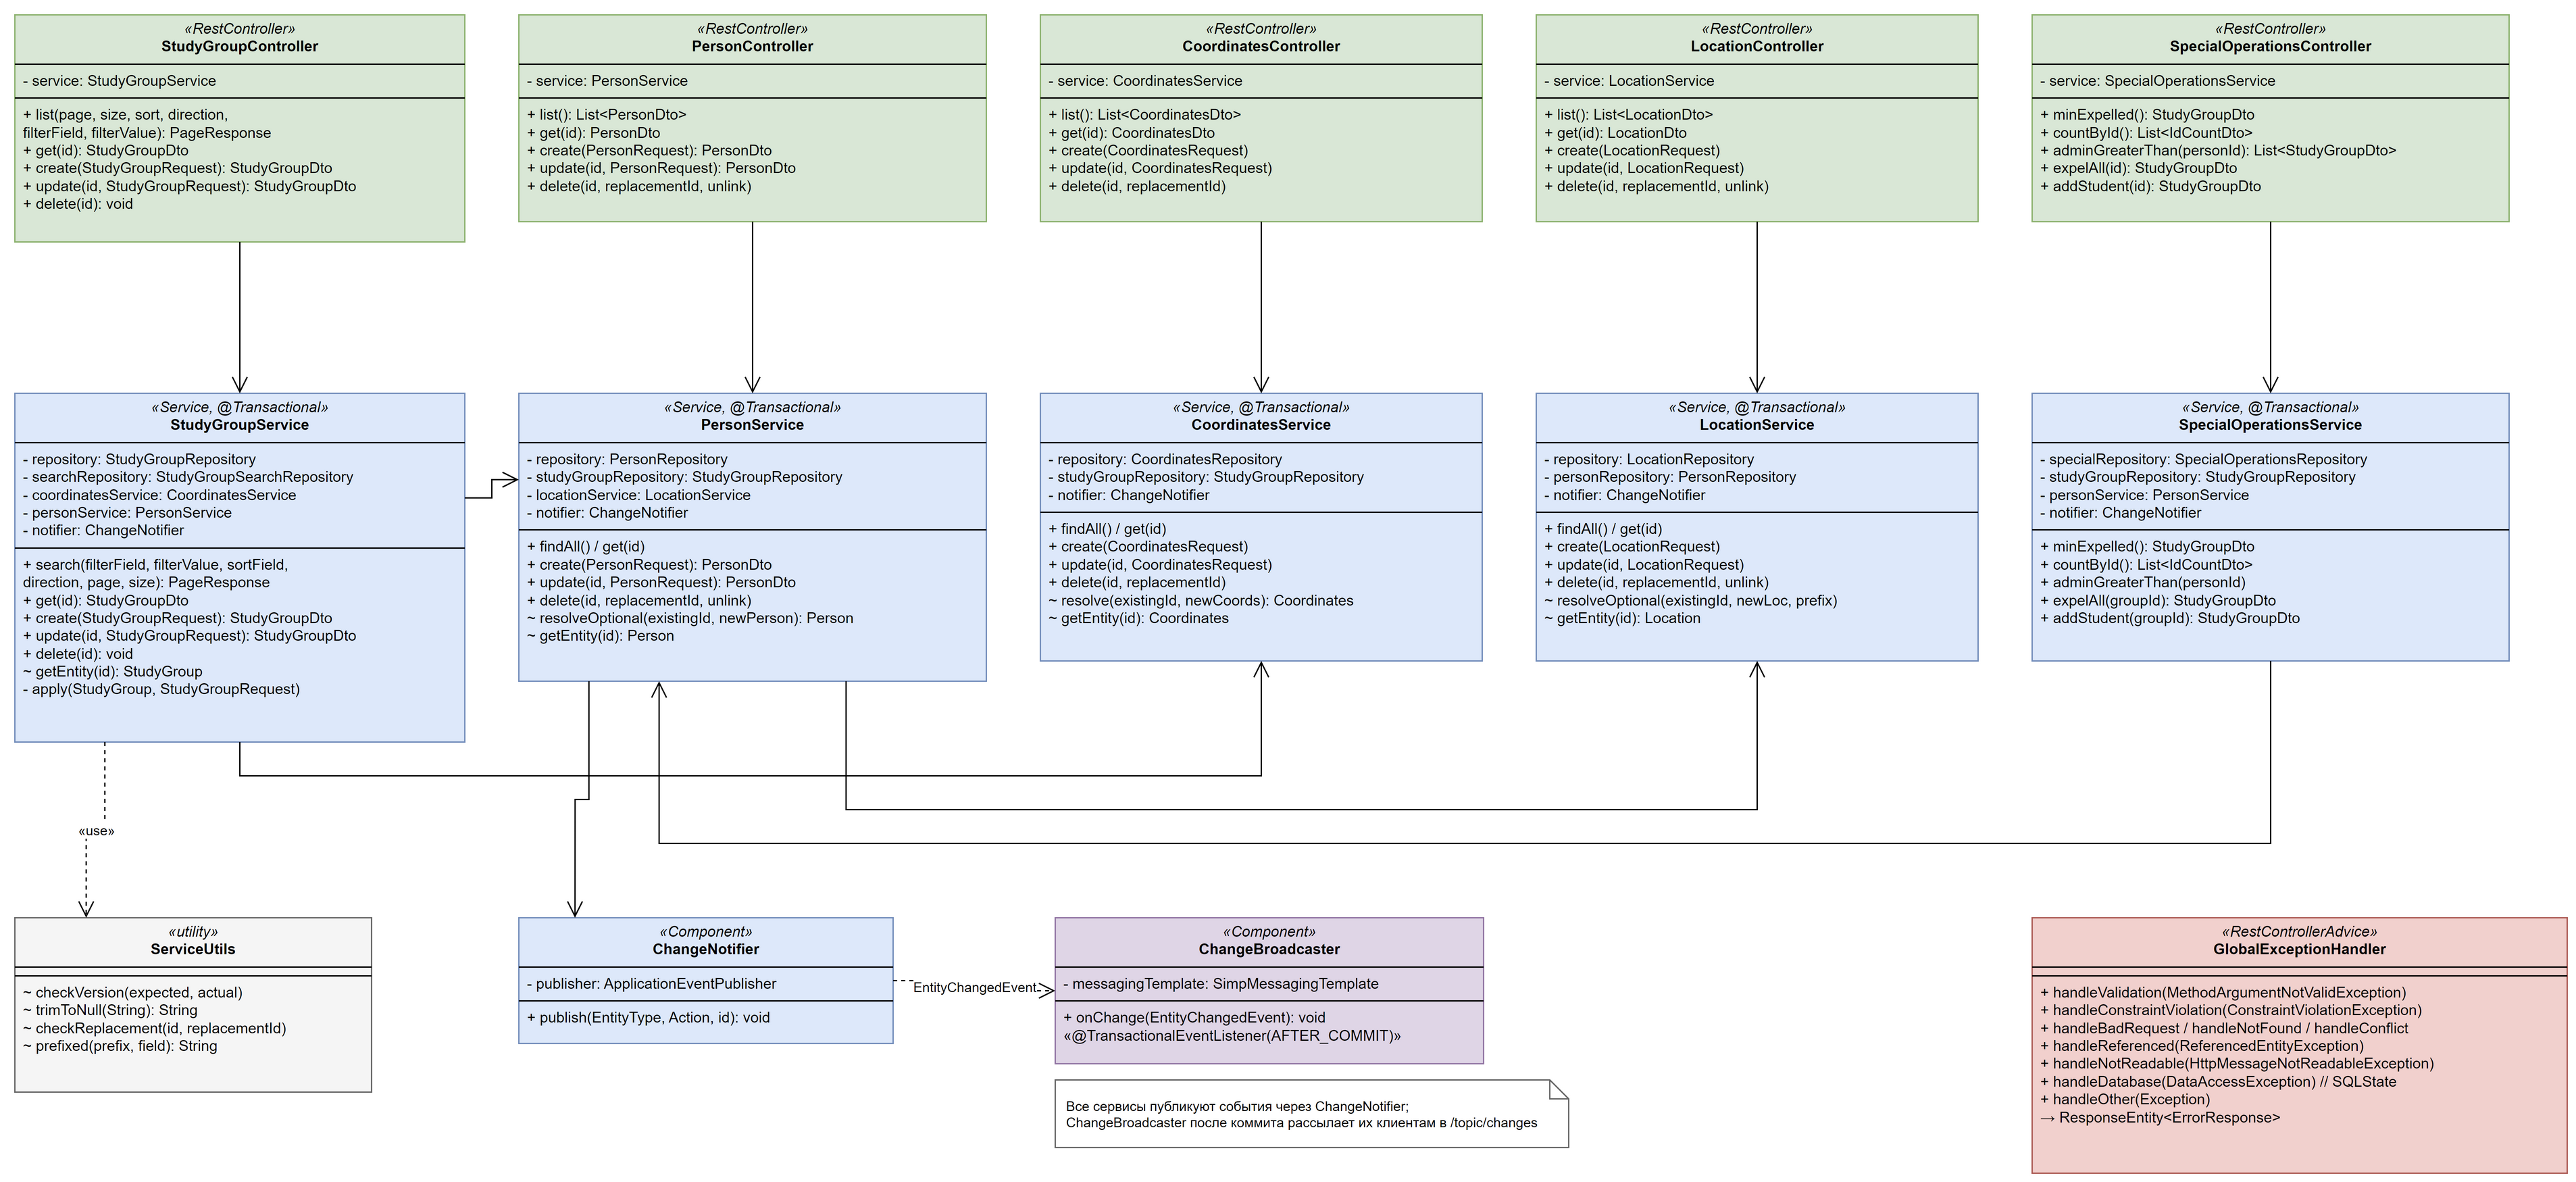
\includegraphics[width=\linewidth,height=0.8\textheight,keepaspectratio]{images/uml-3.png}
  \caption{Диаграмма классов: контроллеры и сервисы (пакеты \texttt{web}, \texttt{service}, \texttt{realtime})}
  \label{fig:services}
\end{figure}

\begin{figure}[p]
  \centering
  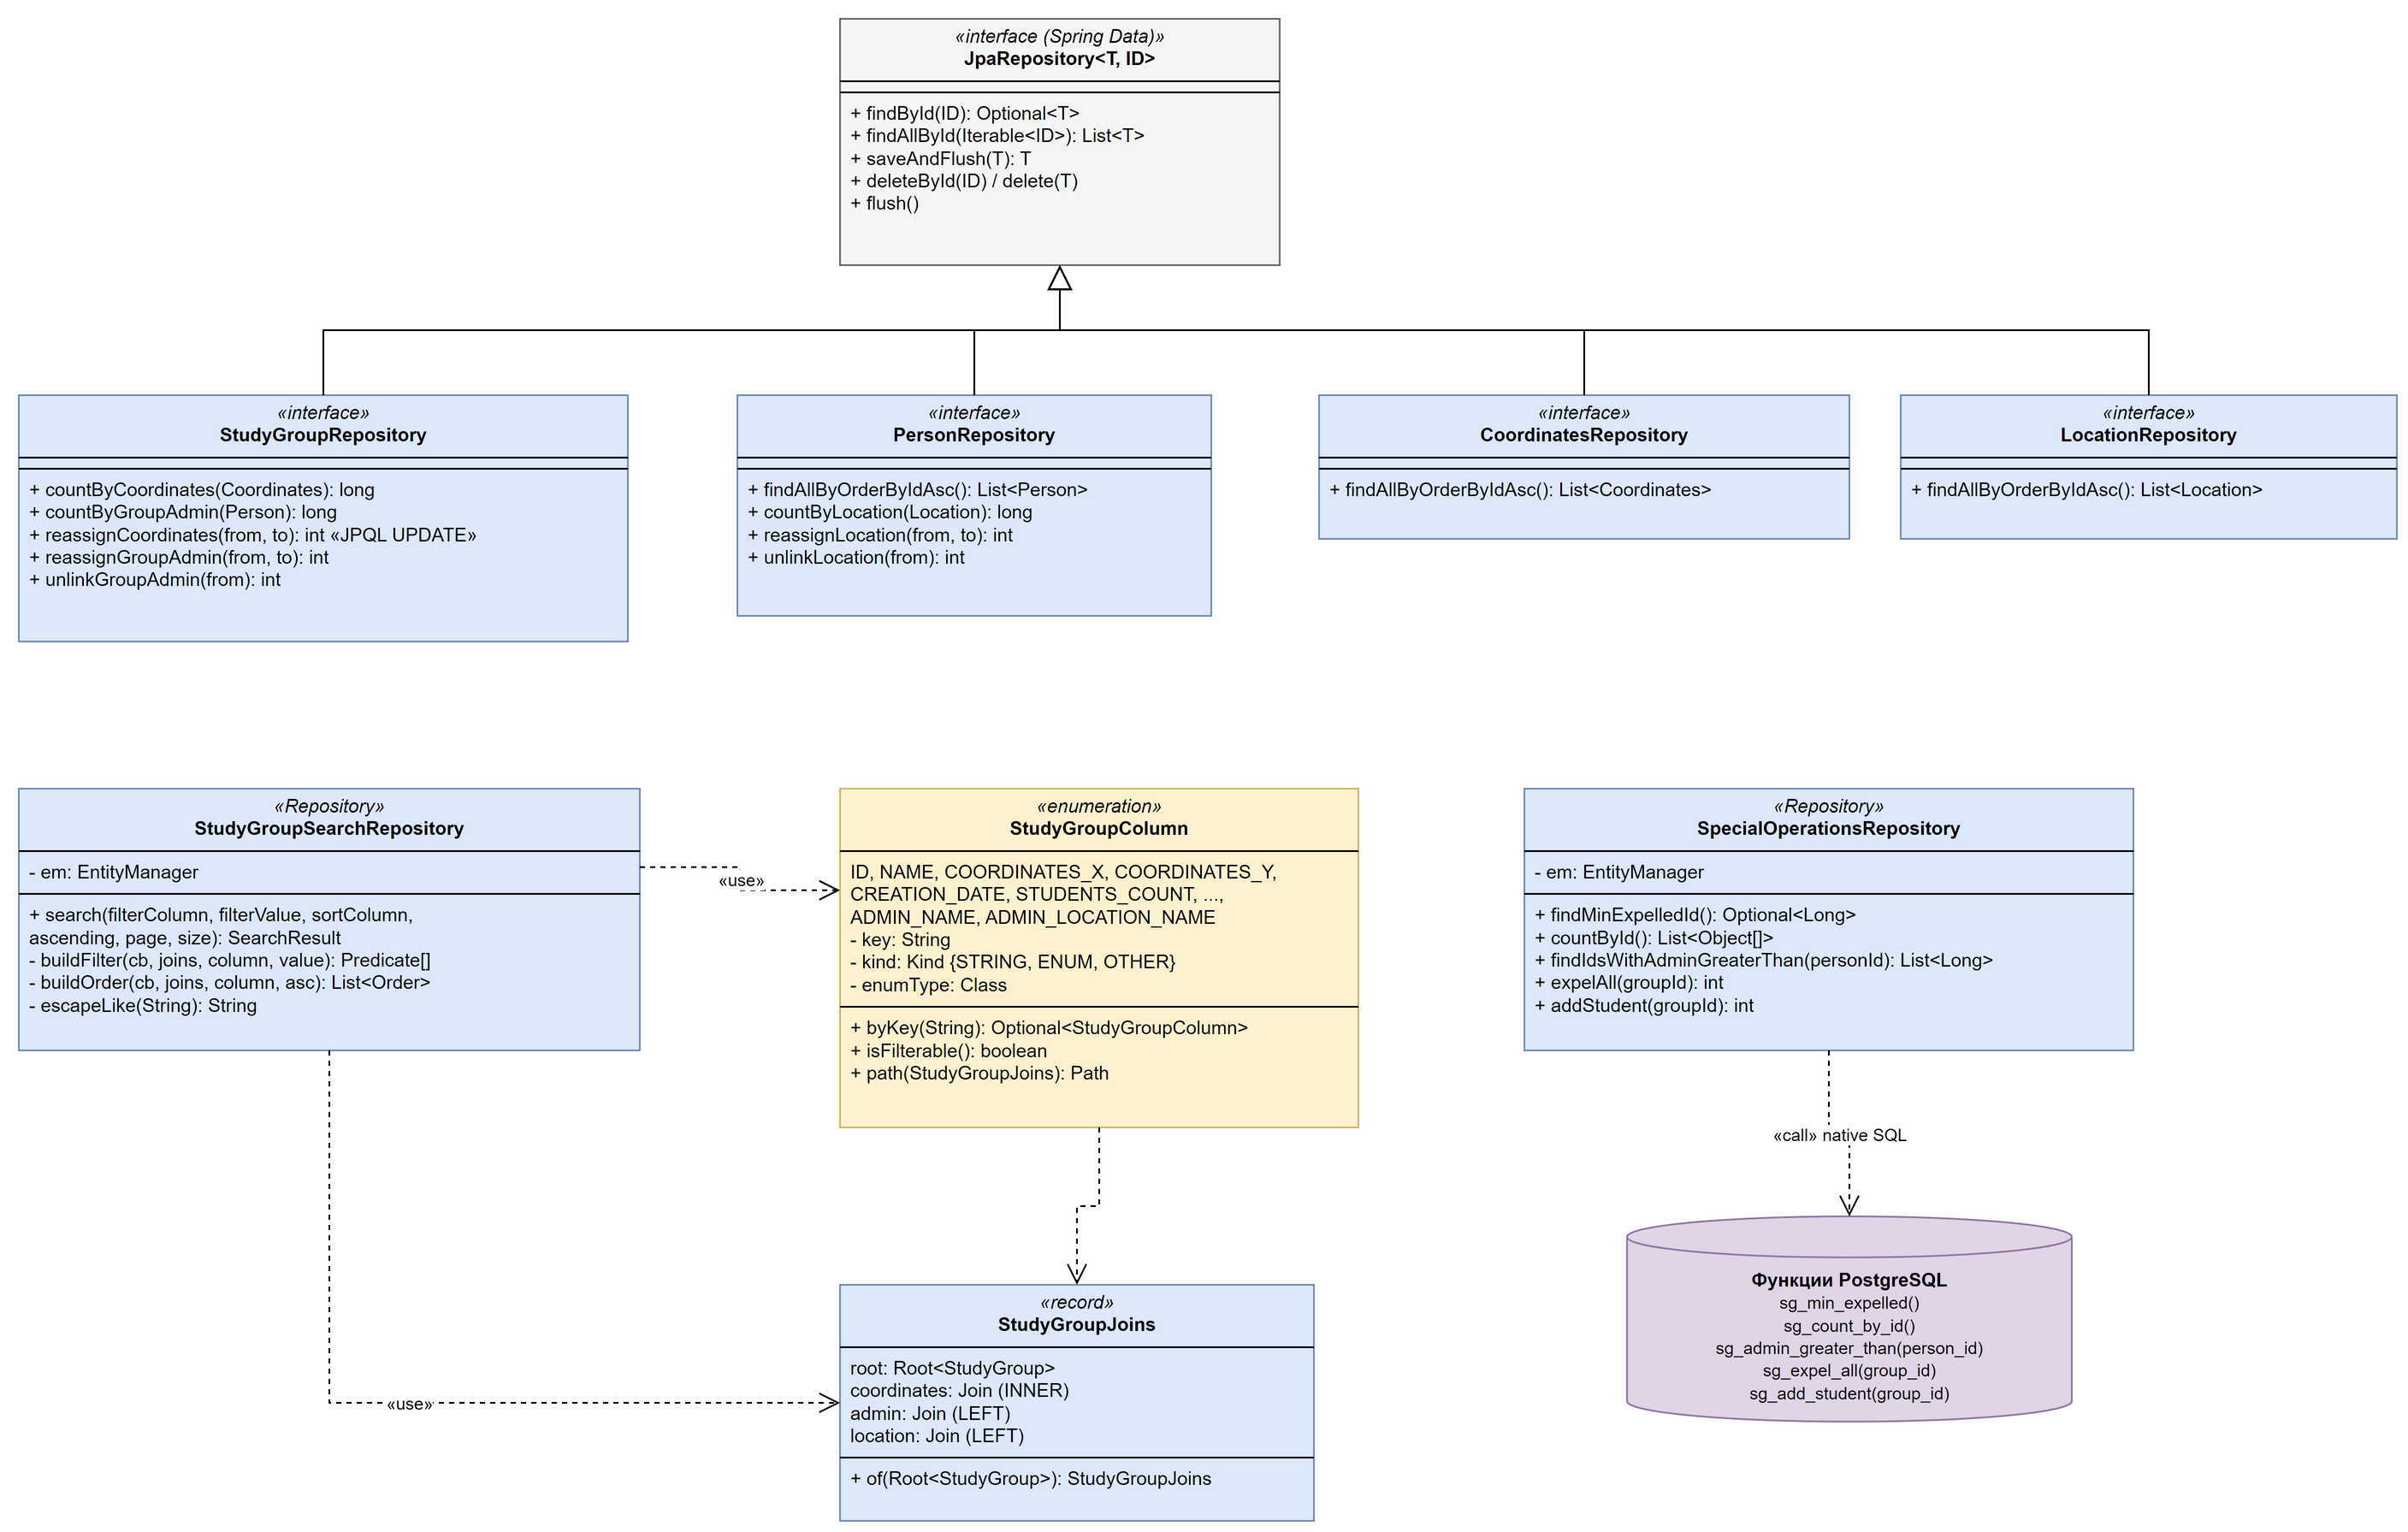
\includegraphics[width=\linewidth,height=0.8\textheight,keepaspectratio]{images/uml-4.png}
  \caption{Диаграмма классов: уровень хранения (пакет \texttt{repository})}
  \label{fig:repository}
\end{figure}

\begin{figure}[p]
  \centering
  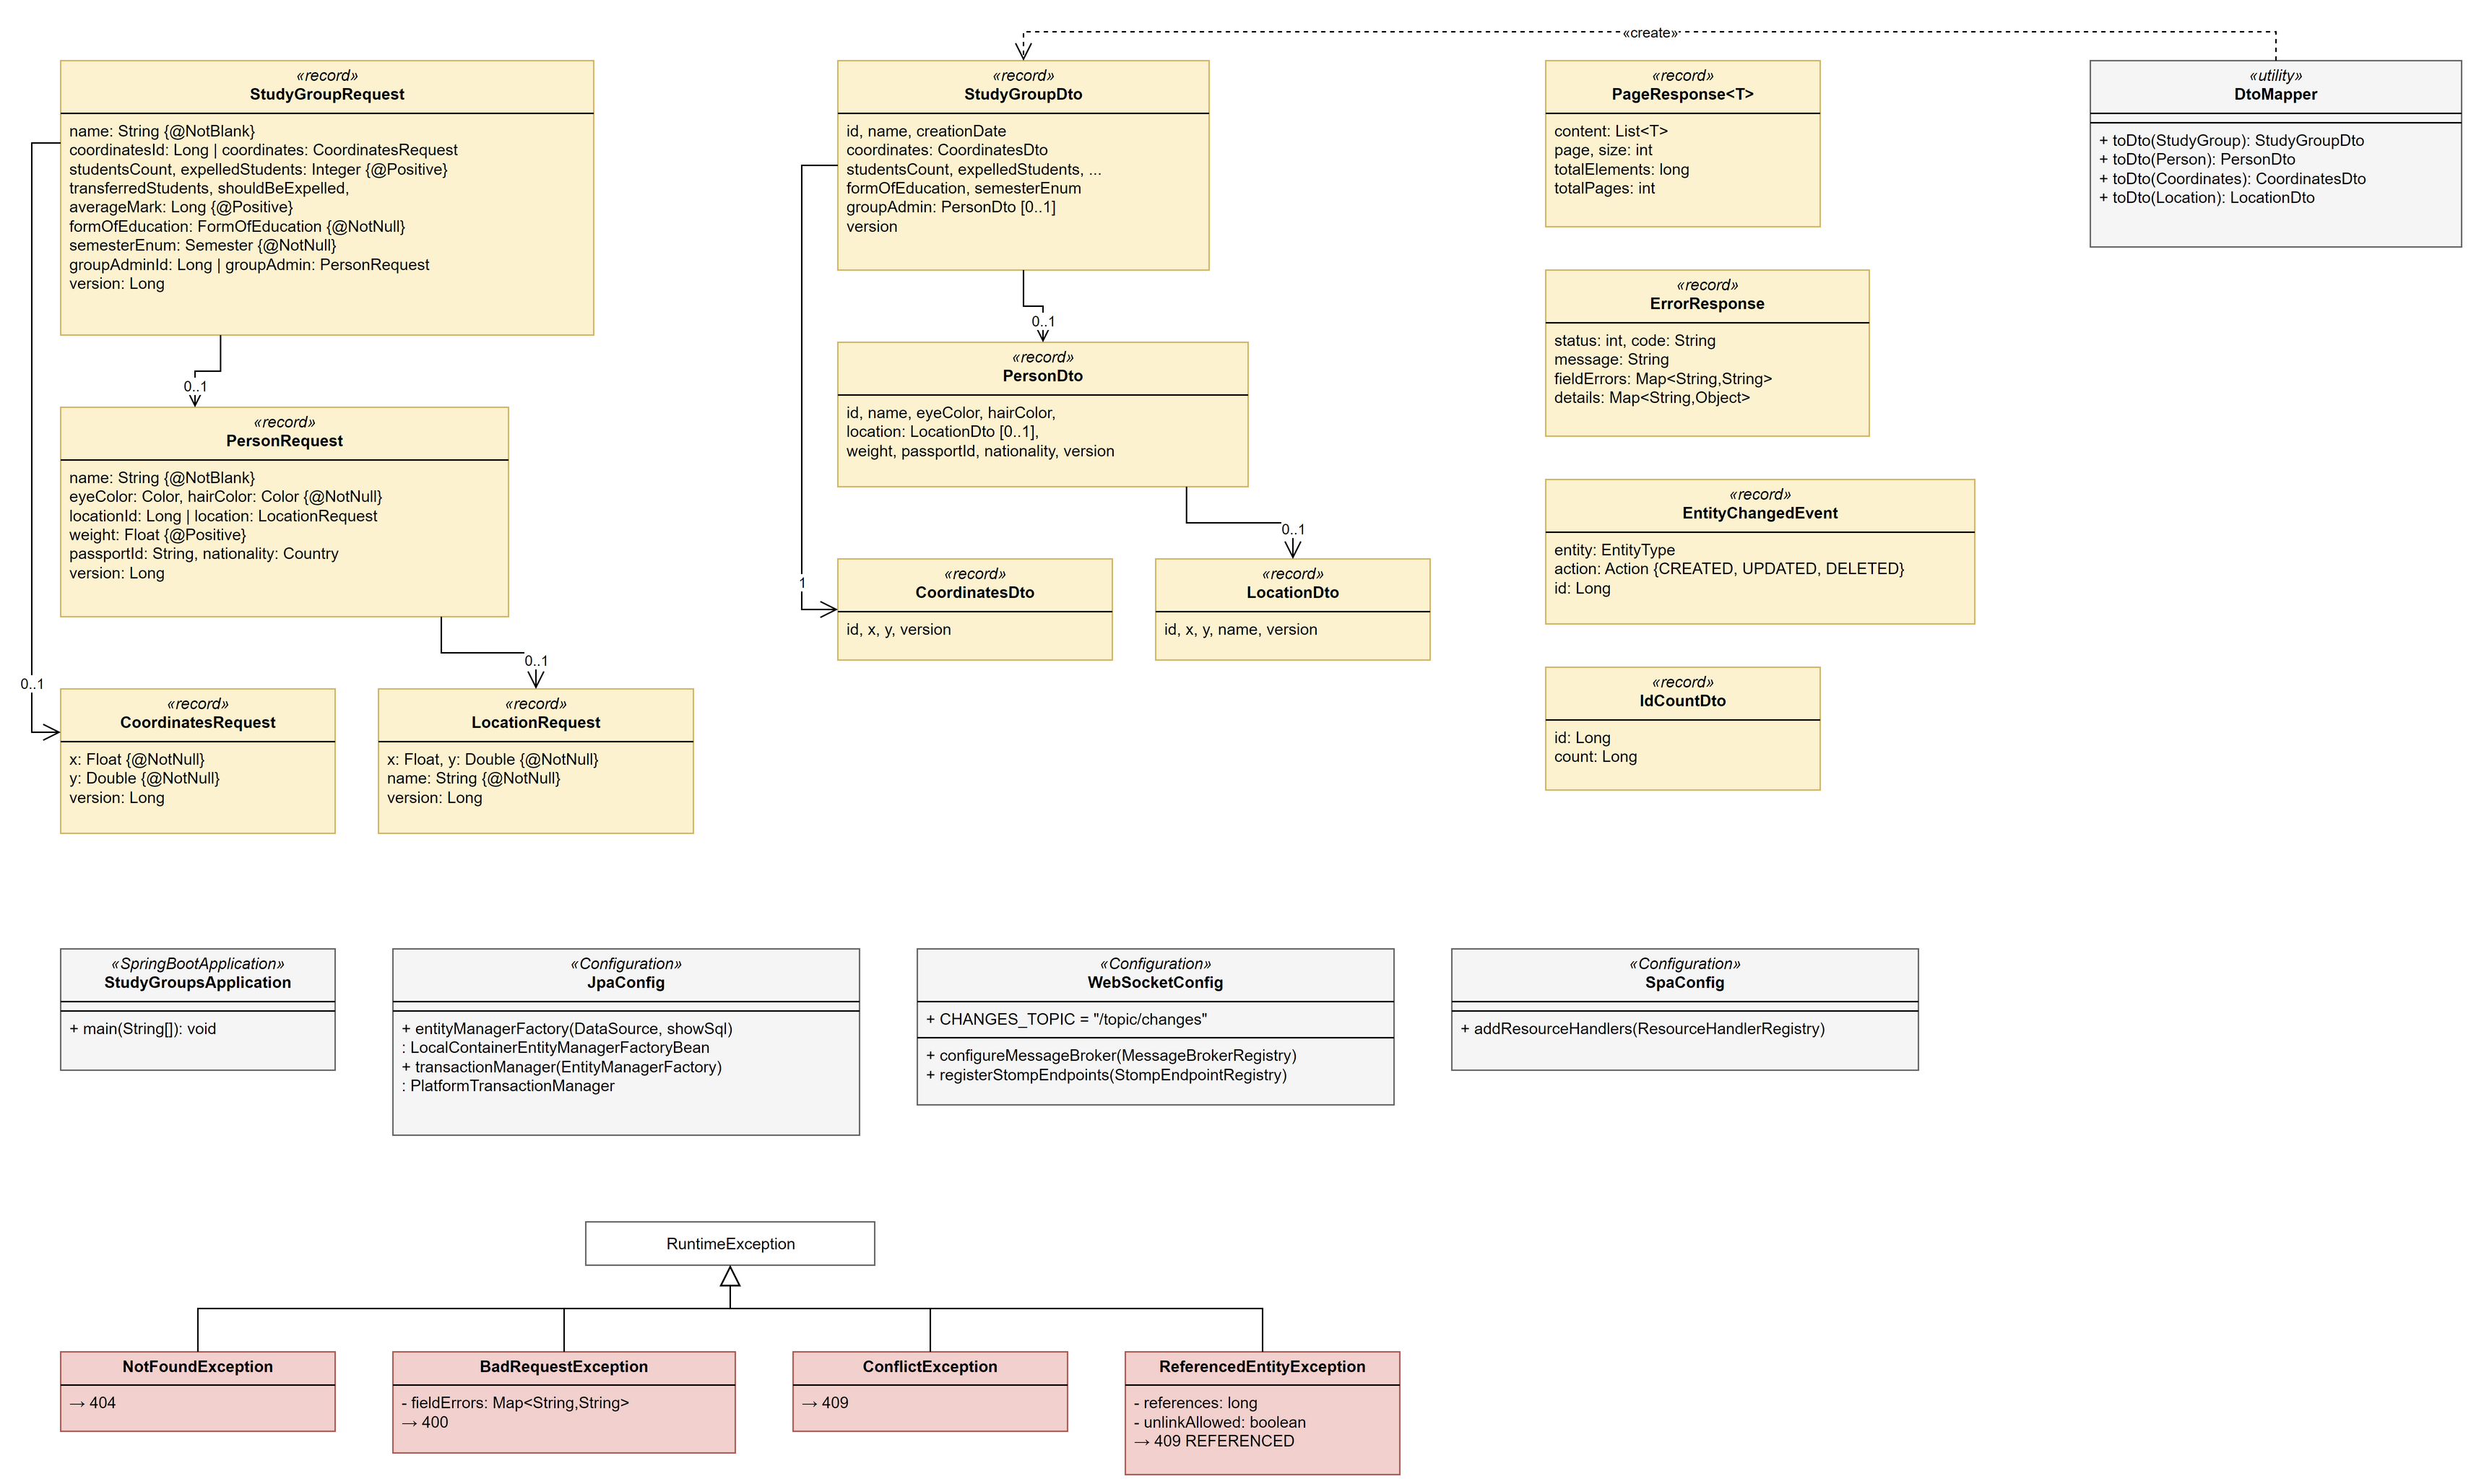
\includegraphics[width=\linewidth,height=0.8\textheight,keepaspectratio]{images/uml-5.png}
  \caption{Диаграмма классов: DTO, конфигурация, исключения (пакеты \texttt{dto}, \texttt{mapper}, \texttt{config}, \texttt{exception})}
  \label{fig:dto}
\end{figure}
\end{landscape}

\subsection{Реализация требований}

\begin{table}[H]
\centering
\small
\begin{tabularx}{\textwidth}{>{\raggedright\arraybackslash}p{0.34\textwidth} >{\raggedright\arraybackslash}X}
\toprule
\textbf{Требование} & \textbf{Реализация} \\
\midrule
CRUD в отдельных окнах & Страницы «Создать группу», «Поиск по ID»; модальные окна редактирования и удаления \\
Информация о связанных объектах & \texttt{StudyGroupDto} содержит координаты и администратора с его локацией \\
Связь с существующими объектами & В форме для каждого связанного объекта выбор: «существующий / новый / не задан» \\
Таблица с пагинацией, фильтрацией и сортировкой & Серверная пагинация; Criteria API, \texttt{LIKE '\%...\%'} без учёта регистра; белый список колонок \\
Обновление у всех клиентов & \texttt{ChangeNotifier} $\to$ \texttt{ChangeBroadcaster} (после коммита) $\to$ STOMP $\to$ перезапрос данных на клиенте \\
Удаление связанного объекта & Ответ 409 \texttt{REFERENCED} $\to$ выбор объекта-замены или отвязка $\to$ \texttt{UPDATE} ссылок и \texttt{DELETE} в одной транзакции \\
Сообщения об ошибках ввода & Проверки на клиенте, \texttt{@Valid} для DTO, Bean Validation сущностей, \texttt{CHECK} в БД; ошибки возвращаются по полям \\
Специальные операции & Функции PostgreSQL \texttt{sg\_*}, вызываемые из \texttt{SpecialOperationsRepository} \\
Одновременное редактирование & Оптимистическая блокировка (\texttt{@Version}), ответ 409 при конфликте \\
\bottomrule
\end{tabularx}
\caption{Соответствие требований и реализации}
\end{table}

Принятые решения по неоднозначным формулировкам специальных операций:
\begin{itemize}
  \item «Отчислить всех студентов группы»: все студенты добавляются к отчисленным, а \texttt{studentsCount} и \texttt{transferredStudents} становятся равны 0. Для этих двух полей ограничение в БД и в сущности ослаблено до $\geq 0$ (миграция V3), при вводе пользователем по-прежнему требуется значение больше 0.
  \item «\texttt{groupAdmin} больше заданного»: объекты \texttt{Person} сравниваются лексикографически по паре \texttt{(name, weight)}; группы без администратора не учитываются.
  \item «Сгруппировать по \texttt{id}»: \texttt{id} уникален, поэтому каждая группа содержит ровно один элемент.
\end{itemize}

\newpage
% =====================================================================
\section{Исходный код системы}

Полный исходный код системы доступен в репозитории: \url{\repourl}.

Ниже приведены ключевые фрагменты.

\lstinputlisting[language=PGSQL, caption={Схема базы данных (V1\_\_schema.sql)}]{code/V1__schema.sql}

\lstinputlisting[language=PGSQL, caption={Изменение ограничений (V3\_\_allow\_zero\_after\_expel.sql)}]{code/V3__allow_zero_after_expel.sql}

\lstinputlisting[language=PGSQL, caption={Функции специальных операций (R\_\_special\_operations.sql)}]{code/R__special_operations.sql}

\lstinputlisting[language=Java, caption={Сущность StudyGroup (поля и отображение на таблицу)}, firstline=1, lastline=80]{code/StudyGroup.java}

\lstinputlisting[language=Java, caption={Настройка EclipseLink (JpaConfig.java)}]{code/JpaConfig.java}

\lstinputlisting[language=Java, caption={Бизнес-логика групп (StudyGroupService.java)}]{code/StudyGroupService.java}

\lstinputlisting[language=Java, caption={Удаление с перепривязкой (PersonService.java)}]{code/PersonService.java}

\lstinputlisting[language=Java, caption={Вызов функций БД (SpecialOperationsRepository.java)}]{code/SpecialOperationsRepository.java}

\lstinputlisting[language=Java, caption={Рассылка изменений клиентам (ChangeBroadcaster.java)}]{code/ChangeBroadcaster.java}

\lstinputlisting[language=TypeScript, caption={Подписка клиента на изменения (useRealtime.ts)}]{code/useRealtime.ts}

\newpage
% =====================================================================
\section{Выводы}

В ходе выполнения лабораторной работы была разработана информационная система для управления объектами класса \texttt{StudyGroup} и связанными с ними объектами \texttt{Coordinates}, \texttt{Person} и \texttt{Location}.

Серверная часть реализована на Spring MVC (Spring Boot 3) с разделением на уровни представления (REST-контроллеры), бизнес-логики (сервисы с декларативными транзакциями) и хранения (JPA + EclipseLink). Так как автоконфигурация Spring Boot поддерживает только Hibernate, фабрика \texttt{EntityManagerFactory} для EclipseLink была настроена вручную. Схема базы данных и функции специальных операций создаются миграциями Flyway, что позволяет развернуть систему на кафедральном сервере без ручного выполнения SQL-скриптов.

Ограничения на поля классов выполняются на нескольких уровнях: на клиенте для удобства пользователя, при приёме запроса (Bean Validation DTO), при сохранении сущности (Bean Validation в EclipseLink) и в самой СУБД (\texttt{NOT NULL}, \texttt{CHECK}, внешние ключи). Ошибки на любом уровне приводятся к единому формату и показываются пользователю рядом с соответствующим полем формы.

Автоматическое обновление интерфейса у всех пользователей реализовано по схеме «издатель "--- подписчик»: события об изменениях публикуются внутри приложения и рассылаются клиентам по WebSocket только после фиксации транзакции. Это исключает рассылку уведомлений об отменённых изменениях и ситуацию, когда клиент перечитывает данные раньше, чем они попали в базу. Одновременное редактирование одного объекта разными пользователями обрабатывается оптимистической блокировкой.

Специальные операции реализованы в виде функций PostgreSQL и вызываются из уровня бизнес-логики через нативные запросы. Изменяющие функции выполняют атомарное обновление одним SQL-запросом и увеличивают версию записи, поэтому корректно работают при параллельных запросах.

В результате работы были получены практические навыки проектирования многоуровневого веб-приложения на Spring, работы с JPA и EclipseLink, использования средств СУБД для обеспечения целостности данных, а также организации взаимодействия клиента и сервера в реальном времени.

\end{document}
